\documentclass[11pt]{article}
%Gummi|062|=)
\usepackage{graphicx}
\usepackage{pdfpages}
\begin{document}

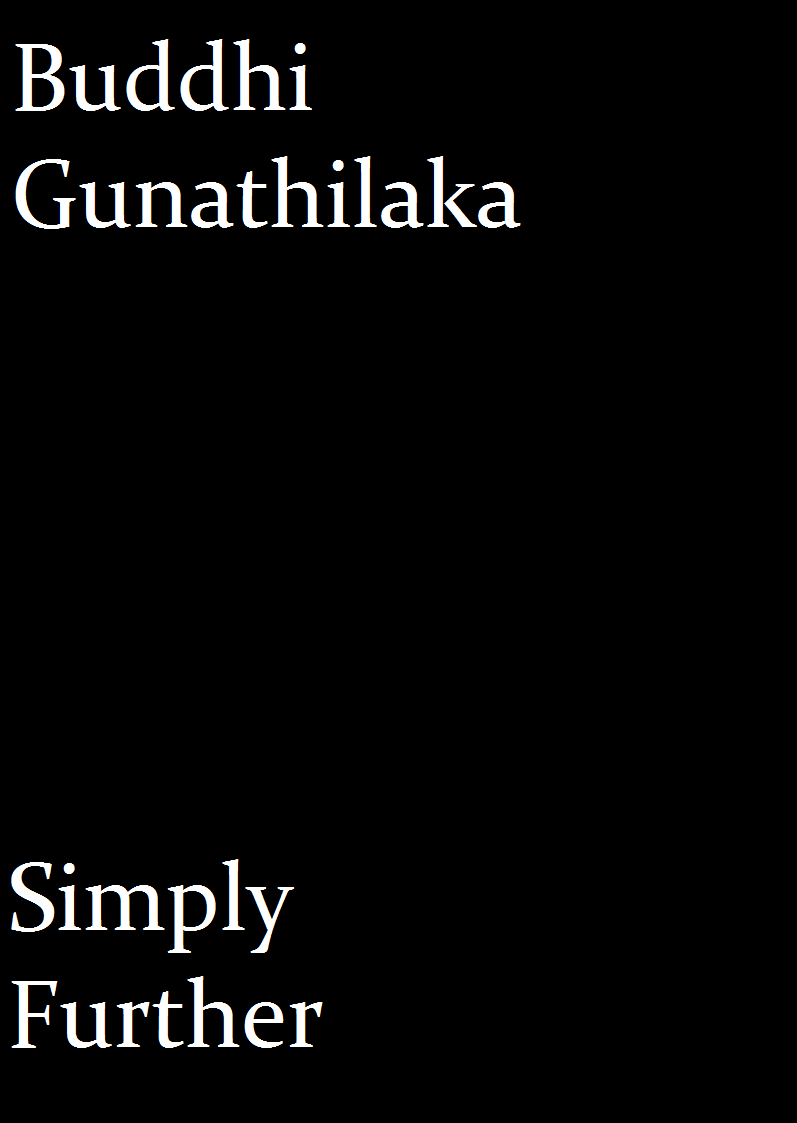
\includepdf{FrontCover(Needswork).png}
\section*{Introduction}

\emph{'Maths ain't easy'.}

I used to be bad at maths. Maybe I still am, I dont' know. Thankfully, the kids I teach seem to be pretty good at Further, so that means I must be doing something right.

That's why I wrote this book, in order to help others who arent' doing that great at maths. I've tried to write this book so that anyone can just pick it up and read through, and find out what they're confused about. 

If you've got any questions, hit me up on the site. Corrections/Additions the same.
 
Let's get started.

\section*{Background}
Further Mathematics is considered by many to be the easiest of the three units you can take at the VCE level. That being said, many students often underestimate further as even simple mistakes can be the difference between a really good mark, and an average mark. In combination with this, Further Mathematics is the second most popular subject in VCE (according to VCAA), so every mark counts. 

The way this book will work is that it'll be seperated into different sections. The first section will be called \textbf{core} and will contain the maths that every further student should know and comprises a large section of the exam. The next sections will be split up into different \textbf{modules}, as each student (or school) is allowed to pick seperate modules to study, so each further curriculum for one school might be different to that of another school. 

Lastly, there'll be a small section of the most common mistakes that occur in further, and some tips and tricks to help you out throughout the year. Feel free to read this book in whatever order you feel free, although keep in mind some chapters may continue on from previous ones. 

\section*{Acknowledgements}
A quick shout-out to LaTex, which is what I wrote this book in. For those who are interested, I wrote it in Gummi (\emph{For Windows}) and it was vey helpful in getting the book set out the way it is. Also, thanks to my girlfriend, who had to put with my continous complaining that I never started to write this book. You're the best! And finally, to you, thanks for reading this and I hope you find it useful.

\newpage

\section*{Core (Data Analysis)}
\subsection*{\underline{Univariate Data}}
\subsubsection*{Data Types}
There are multiple types of data that you will explore in further maths. These three types are called \emph{univariate}, \emph{bivariate} and \emph{multivariate} data. Now to the uninitiated, these terms would probably mean absolute gibberish, however the meanings are quite simple. 'Univariate' data means data that only has one \underline{variable} (read: something that changes over time. An example of this is the number of books a bookstore sells, since it is a singular number (i.e 50 books sold), it would fall under the univariate data category. 

In comparison, 'bivariate' data means data that has two variables. A simple way to remember the difference is that univariate data starts with 'uni', or latin for one (like unicyle, with one wheel) and bivariate which starts with 'bi', which is latin for the number two (bicycle = two wheels). A good example of bivariate data is the avaerage age of a worker and the salary that he makes. We'll talk about bivariate data later on.

There are also multiple different categories that we can place data into, which further helps distinguish data in order to make it easier to read and gain information from. The first way to categorize data is by seeing if it is \emph{numerical} or \emph{categorical}. Basically, if the data is in numerical form, it falls into the numerical category (duh!). Examples like 50 cows, 27 monkeys, 136 cars, one hat are all examples of numerical data. On the other hand, categorical data is basically data that cannot be expressed in numbers. If a deem a person male or female, that data can't be represented by numbers, although I can write down Male or Female. The same goes for teams, sports, cars etc. Ratings also fall under this catergory as well, for example if I give a cake that my girlfriend makes a score of 4/10 (don't kill me!), that would be a catergorical piece of data.

Another way we can categorize data is seeing if it is either \emph{discrete} or \emph{continuous}. A discrete piece of data means that the data can only take a certain fixed set of values. The average family is said to have 2.5 children, but you can't really have half a child. Therefore the amount of children that a family can have is discrete, where it has to be a whole number, and not a decimal. Another of of thinking about it is that if you can count it, it's a discrete piece of data. In comparison, continuous data can be any range of numbers, such as height, which is almost never exactly 1m or 2m, but is someway halfway (for example, I'm 175cm or 1.75m). My height would therefore be a continous piece of data because it is a decimal value, and as such cannot be counted. Seriously, try counting every decimal between 1 and 2, and you'll see what I mean. 

\subsubsection*{Stem Plots}
What is a Stem Plot? It's a way of displaying small sets of data in a way that you can just take a glance at it, and get a quick overview of the complete set. It's used for discrete data (like we mentioned before). Each number that is placed into the stem plot is seperated into the '\emph{stem}' and the '\emph{leaf}'. For example, for the number 21, 2 would be the stem and 1 would be the leaf. So if I wanted to represent another number, say 25, I just have to add a five to the right hand column, as it would share the same stem as the number 21. 

The picture below shows an example of a stem plot and how it is seperated into the stem and leaves.
 
\begin{figure}[htp]
\centering
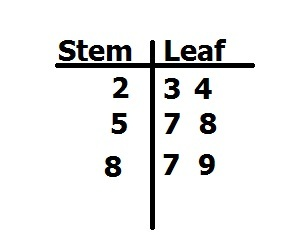
\includegraphics[scale=1.00]{StemLeafImage1.jpg}
\label{}
\end{figure}

As you can see, there are a variety of numbers (23, 24, 57, 58, 87, 89). They've been split up into stems and leaves. From a quick glance, we can tell how many values are within the twenties, or if there is an 87 located in the set, which shows how easy it is to display information within a stem plot. However, there are drawbacks to using a stem plot, the most obvious of which is using large sets of data, where writing it in a stem plot would take hours and would be very confusing. 

However, if you did have to put a large number of numbers (odd wording), you could actually double up on the numbers in the stem column (i.e have two 2's) in order to make the stem plot look simpler. In picture form, we're talking about something like what follows below.

\begin{figure}[htp]
\vspace*{0.5cm}
\centering
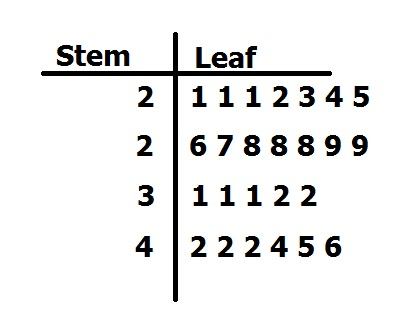
\includegraphics[scale=1.00]{StemLeafImage2.jpg}
\end{figure}

As you can see, the stem section has two 2's. This is because there are so many values in the twenties, it would have probably overflowed and gone off the page. In order to make the stem plot look cleaner, we can split the twenties into two different sections. In this stem plot, we seperated it into two different sections, 20-25 and 26-29. So if you ever find this in a exam or even come across it in a textbook, you can be assured that it isn't someone whos made a typo, but it is a legitimate way to represent stem plots. 

\subsubsection*{Other Ways to Display Data}

Stem Plots aren't the only way to display data in a visual way. Other forms have also been invented in order to make it easier to appreciate data without having to sift through a pile of numbers.

The first of these alternate forms is the \emph{Frequency Table}. The main benefit to a frequency table is that it is used for larger data sets, and shows an easier way to represent data visually without taking up lots of space. Just as an aside, Frequency Table also look like the scratches that people stuck in jail make in tv shows, where they count the days before they're free. An example of it is shown below:

\begin{figure}[htp]
\centering
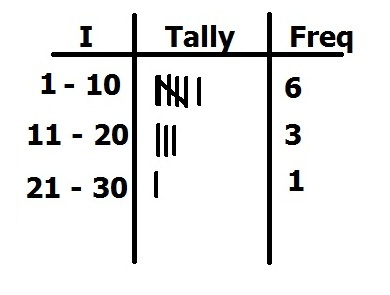
\includegraphics[scale=1.00]{FreqTableImage3.jpg}
\end{figure}

Let's assume we have a friend called Bob. He's just been jailed for tax evasion. The frequency table shown above shows the amount of times he's been served glop in the prison cafeteria in a given period (ten days, Bob's been in so long he doesn't remember what a week is). We can see that in the first ten days, Bob's been served glop 6 times, and in the next two periods, he's been served glop 3 times and one time respectively. In total, he's been served glop 10 times in a 30 day period. That's a lot of glop. 

The frequency table shows a really easy way to actually show all this information, and can be extended further and further, due to each set of five being shown as a seperate symbol. 

Frequency tables are great, but I like pictures. Thankfully, thats where Frequency Histograms come in. They can be used for both discrete and continous numerical data. Many of you would have heard of bar charts, and that is \emph{almost} exactly what a frequency histogram is (It's fancy). Let's take a look at what Bob's glop adventures would look like in picture form.

\clearpage{}
\begin{figure}[htp]
\centering
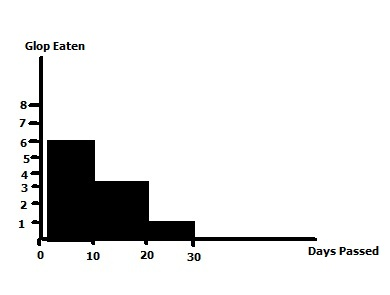
\includegraphics[scale=1.00]{HistoGramImage4.jpg}
\end{figure}

As we can see, the x-axis (you're going to be hearing that one a lot) has the different periods of time that Bob has experienced, while the y-axis (ditto) shows the amount of times Bob has eaten some glop. It's important to note that the bars don't start from \textbf{zero}, they start at one because the first period is shown to be 1-10 as seen in the previous frequency table.

There are other ways to display this kind of data, which each has their own benefits. Another form to display data is called the \emph{dot plot}. This is basically a series of dots placed at intervals above a line which indicates how many data points are associated to one interval. If that just made no sense to you, why don't we just take a look at the diagram instead on the next page?

\clearpage{}
\begin{figure}[htp]
\centering
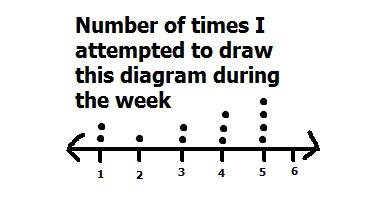
\includegraphics[scale=1.00]{DotPlotImage5.jpg}
\end{figure}

Each day has a certain amount of dots above to indicate how many times I tried to draw the diagram on that specific day. As we can see, I got that diagram way too many times, and towards the end of the week, I attempted to draw it a lot more than at the start of the week. Pretty simple. Keep in mind, I could actually change the numbers to actual days and the plot would still make sense.

By extention, we now know how bar charts work, as they are very similar to frequency histograms, although they can actually start at zero as some data given may start with an initial value of zero. Otherwise, bar charts are almost indistinguishable from frequency histograms.

There's other information we need to know in order to complete our knowledge of frequency histograms, and that is how we can describe the data we see in a histogram visually. By this I mean that the graph takes on a certain pattern which can clue us into what kind of data we're looking at. The four kinds of patterns that we're looking at is shown below:

\begin{figure}[htp]
\centering
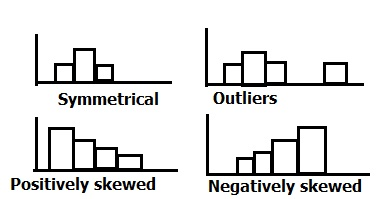
\includegraphics[scale=1.00]{SkewedImage6.jpg}
\end{figure}

These pretty much show what the data is trying to tell us. A symmetrical histogram is usually saying that the data is building up to a peak point then then dropping again (or the other way around). Outliers (which are important later on) show pieces of data which doesn't fit the normal pattern seen with the data. Lastly, positively skewed and negatively skewed data show that the data given is trending in a particular direction. If the data is positively skewed, the data starts off on at a high point and reduces over time. On the other hand, if the data is negatively skewed, then the data starts off small and increases over time.

\subsubsection*{Median, IQR, Range and Mode}
Now that we've got a visual representation of data down pat, we can start to look at ways to obtain statistics from data. The statistics we gain from data is important in many different fields, and chances are when you get past high school, you'll still be using it. So pay attention!

The first statistic we can look at is the \emph{median}. Contray to popular opinion, the median is very different to the \emph{mean}, which we'll take a look at later. The median is simply the \emph{middle} number. For example, if we had a set of five numbers:
\begin{displaymath}
1, 2, 3, 4, 5
\end{displaymath} 
The middle number and therefore the median is 3.
But what happens if there isn't any middle number? Let's take a set of six numbers.
\begin{displaymath}
1, 2, 3, 4, 5, 6
\end{displaymath}
Then the middle number lies in between 3 and 4, because that is the 'middle' of the entire set. In this example, that number, and median would be 3.5. Pretty easy to remember!

The second statistic that we should cover is the range. The range is pretty simple to remember, in that you just have to subtract the lowest value in the set from the highest value, which gives the range of values that the set covers. For example:
\begin{displaymath}
1, 2, 3, 4, 5, 6
\end{displaymath}
Is our set from before. Let's find out what the range is:
\begin{displaymath}
6 (highest value) - 1(lowestvalue) = 5(range)
\end{displaymath}
As I said before, isn't too hard to remember.

So what is our third statistic? It's called the \emph{mode}. The mode is the number that occurs the most, otherwise known as number with the highest frequency. Let's take a look at another number set and see what we mean:
\begin{displaymath}
1, 2, 3, 3, 3, 5, 6, 6
\end{displaymath}
In this set, the mode is quite clearly 3. How come? Cause it shows up the most in the set.

The final statistic that we should remember is the IQR, or by its full name, it is known as the interquartile range. What is the interquartile range, and additionally, what on earth is a quartile?

An quartile is a quater, what you get when you take something and seperate it into four pieces. The same applies to data, where if we seperate it into four parts, each part would be a quartile, where the middle quartile (Q2) is the median. Therefore, we define the IQR as the third quartile minus the first quartile or the middle 50\% of all the values. The equation (for those of you who like equations) is as follows:
\begin{displaymath}
IQR = Q3 - Q1
\end{displaymath}
 
Now, I know you're pretty confused as to whats going on, and I don't blame you. However, since I like showing you things, bear with me while I explain one more important thing, which will help us to understand the IQR a little better.

\subsubsection*{Boxplots}

What is this important thing? \emph{Boxplots}. What is a boxplot? A nice little diagram from which we can see all the different information we just covered! It'll also be something that you'll spend a lot of time drawing, so let's take a closer look at it (on the next page)!

\clearpage{}
\begin{figure}[htp]
\centering
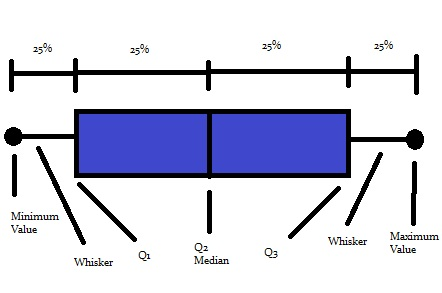
\includegraphics[scale=1.00]{IQRImage7.jpg}
\end{figure}

There are a few interesting things we can see in this diagram. We can see that there are clear quartiles with the box plot, with each section representing a quarter. Also, the blue section represents the IQR, as it is the difference between Q3 and Q1, or the space in between the two. The median is also known as Q2, and the minimum and maximum values are where the boxplot starts and ends. That's a lot of information!

Now we understand how to read a boxplot, we're going now work out how to draw one. Let's start with our trusty set of data:

\begin{displaymath}
1, 2, 3, 3, 3, 4, 5
\end{displaymath}

We need to work out a few things in order to draw the box plot, let's start with where the boxplot starts and ends. We know from the diagram that the boxplot starts with the minimum value and it ends with the maximum value. So with a careful observation of the data set we've been given, we know the boxplot starts at 1 and it ends at 5, and this is where we draw our whiskers from.

\begin{displaymath}
Minimum \; value: 1
\; Maximum \; value: 5
\end{displaymath}

We should now attempt to figure out where Q2 is, or the median. Now for those who've been paying attention, we know that the median is simply the middle number! Therefore a quick look at the data set tells us that 3 is our median. 

\begin{displaymath}
Median: 3
\end{displaymath}

One last thing we've got to do, before we draw up our boxplot. We need to figure out what Q1 and Q3 are. Now this is interesting, in that there isn't a obvious way that we can find out what Q1 and Q3 are from looking at the boxplot. This calls for a bit of thinking. We know the middle number or median is 3, and we know that the start point is 1, so therefore we can take the median of the numbers between 1 and the median in order to find Q1. So let's take a look at the numbers I'm talking about:

\begin{displaymath}
1, 2, 3, 3
\end{displaymath}

As we can see, we've got a set of four numbers here, with the median at the far right and the minimum value at the far left. So, using our knowledge of the median, we just find the middle number, which in this case is in the middle of 2 and 3, which gives us the value of 2.5. Therefore, we now know that:

\begin{displaymath}
Q1 \; is \; 2.5
\end{displaymath}

In order to find the value for Q3, we just have to take a look at the data values to the right of the median, including the median itself. Let's take a look at that set of data now:

\begin{displaymath}
3, 3, 4, 5
\end{displaymath}

So let's just do what we did before. We know the median would lie between the two middle numbers, so that gives us a figure of 3.5. This means that

\begin{displaymath}
Q3 \; is \; 3.5
\end{displaymath}

We've now got enough information to draw our boxplot! Let's take a look and see what that looks like on the next page:

\clearpage{}
\begin{figure}[htp]
\centering
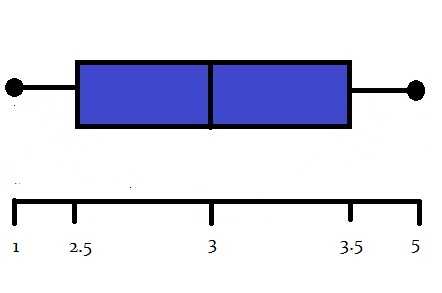
\includegraphics[scale=1.00]{IQRCompleteImage8.jpg}
\end{figure}

\subsubsection*{The mean}
Finally, we get to the mean. This is most likely the easiest thing to remember, cause chances are that you've most likely used it before. The mean is simply the average. Say we've got a data set (another one!):

\begin{displaymath}
1, 2, 3, 4, 5, 5, 6
\end{displaymath}

In order to find the mean, we first add up all the numbers,

\begin{displaymath}
1 + 2 + 3 + 4 + 5 + 5 + 6 = 26
\end{displaymath}

and then divide it by the amount of numbers in the set:

\begin{displaymath}
26/7 = 3.71
\end{displaymath}

And therefore, our mean is 3.71

The mean is great for data sets that aren't skewed, in order to get a good idea of what the middle is, but if you've got a data set thats skewed in a direction, you'll find that the mean gets more inaccurate. Let's see an example.

Let's take a dataset:

\begin{displaymath}
1, 1, 1, 1, 1, 1, 1000000.
\end{displaymath}

Adding up all the numbers gives us the value 1000006. Now if we divide this by the amount of numbers in the set, we can find that the average is 142858. It's pretty obvious that this isn't actually indicative of what the actual middle of the set is as it's heavily skewed in a certain direction. In cases like this, the median is a better inidicator for the middle, with the median being 1, which is a lot more accurate when determining the middle.

\subsubsection*{The Standard Deviation}

So now that we know what the mean means (pardon the pun), we should also find out what the standard deviation is, as the mean and standard deviation is the two most common things you'll see when working with data. So what is the standard deviation? It's basically a way to see how data is spread around the mean. More to the point, its a way to tell how far a point is from the mean, the higher the standard deviation is, the further away from the mean it is. 

How do we work out the mean? Luckily for us, there is a simple formula which lets us plug in numbers and get out a nice number to called the standard deviation (or SD for short):

\begin{displaymath}
s = \sqrt{\frac{\sum (x - \bar{x})^{2}}{n-1}}
\end{displaymath}

Now that may look like a confusing jumble of symbols, but lets break it down and get a heads up on what it all means. 

S is pretty simple, it stands for the standard deviation. But whats this crazy symbol mean?

\begin{displaymath}
\sum
\end{displaymath}

That symbol stands for 'sum of'. So if we had a series of data points under the title 'Series of data points', and we wanted to write 'Add all of series of data points', we would write:

\begin{displaymath}
\sum Series \; of \; number \; points
\end{displaymath}

With regards to the standard deviation, the sum of symbol is saying that we have to add up all the values in the brackets as there are multple values of x in a data set.

But what does the following symbols in the brackets mean?:
\begin{displaymath}
(x - \bar{x})^{2}
\end{displaymath}

This is referring to X, the values in the data set, and the x with a bar over it is the mean. So if you see an equation that has a x with a bar over it, that symbol means the mean. (So many puns!)

Lastly, we need to figure out what this means:
\begin{displaymath}
n-1 
\end{displaymath}

This is just referring to the number of data points, so all you really have to do is is count up how many data points there are and then you've got n. Don't forget to minus one from it though!

So let's put together all that we've learnt, and do a sample question to make sure we know what the heck we're doing.

Say we've got a series of numbers:
\begin{displaymath}
1, 2, 3, 4, 5 
\end{displaymath}
and we're going to find out what the standard deviation is.

First off, let's calculate the mean:
\begin{displaymath}
\bar{x}= \frac{1 + 2 + 3 + 4 + 5}{5} = \frac{15}{5} = 3
\end{displaymath}
Now, we've got to find the \underline{sum of} x subtract the mean, and square the values:

\begin{tabular}{|c|c|c|c|}
\hline
	X & Mean & X - Mean & X - Mean Squared\\
\hline
	1 & 3 & -2 & 4\\
\hline
	2 & 3 & -1 & 1\\
\hline
	3 & 3 & 0 & 0\\
\hline
	4 & 3 & 1 & 1\\
\hline
	5 & 3 & 2 & 4\\
\hline
\end{tabular}

So the \underline{sum of} X - Mean squared would be:

\begin{displaymath}
\sum (x- \bar{x})= {4 + 1 + 0 + 1 + 4} = 10
\end{displaymath}

So, now all we have to do is put this value over (n - 1), and since we know that there is five data points, we can just:

\begin{displaymath}
s = ^{\sqrt{\frac{10}{5-1}}} = ^{\sqrt{\frac{10}{4}}} = 1.581
\end{displaymath}

Which gives us a standard deviation of 1.581. So there are a lot of steps involved, but by going through it one 'block' at a time, you can solve any standard deviation question you set your mind to.

\subsubsection*{The 68-95-99.7\% rule}

Understanding the 68-95-99.7\% rule requries us to know a bit about the bell curve, so let's start with that. 

The bell curve is a nice looking graph which represent about 95\% of all data you'll ever see in your life. What does it look like?

\begin{figure}[htp]
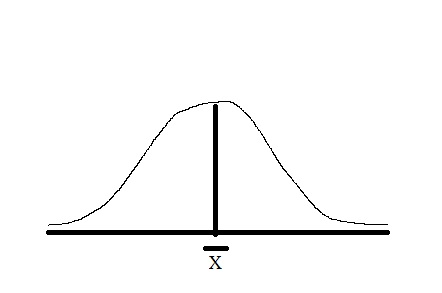
\includegraphics[scale=1.00]{BellCurve1Image9.jpg}
\end{figure}

I left out a lot of detail but you get the general idea. The bell curve slowly increases and reaches its climax at the mean, then it slowly decreases, therefore giving it its bell shape. The reason why this shape is so important is that, like I said before, it represents 95\% of all data you'll ever see. Everything from the distribution of I.Q scores, to the average test marks in a class will follow this pattern, where the vast majority will score around the mean (duh!) and the chance of getting a score (or I.Q score or whatever) decreases when moving further away from the mean.

So where does the 68-95-99.7\% rule come in? To put it in the most simple terms possible, each number refers to the amount of data that lies within a certain amount of standard deviations. So, 68\% is the amount of data that resides within one standard deivation of the mean, 95\% is the amount of data that resides within two standard deviations of the mean and 99.7\% is the amount of data that resides within three standard deviations of the mean. 

So let's put this in graph form:

\clearpage{}
\begin{figure}[htp]
\centering
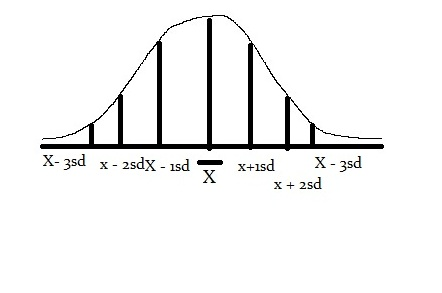
\includegraphics[scale=1.00]{BellCurve2Image10.jpg}
\end{figure}

We can see that the lines correspond to the amount of data localized by the standard deviation. We can also see that the further away the standard deviation is from the mean, the more data we can incoporate. Now the most vital bit to know is that this could correspond to actual data points, so for example we can say that '68\% of people reside between 10 and 20' if 10 and 20 correspond to the mean subtract one standard deviation, and the mean add one standard deviation respectively. 

\subsubsection*{The Z-Score}

Sometimes, when we get score, we want to compare it to other people. Otherwise, a score is meaningless, right? In that line of thinking, when we have a data point, the main point of it is to compare it to other data points. That's where the Z-score comes in. The Z-score is the '\emph{standardised} score, so it can be compared to other scores. So, how do we figure out the Z score? The equation is as follows:

\begin{displaymath}
z = \frac{x - \bar{x}}{s}
\end{displaymath}

We've previously gone over what the symbols mean, so if you get confused, just double back and read over them. It's okay, I'll wait.

Done? Cool, now lets dive into what the z-score means, numerically. A z-score of 0 means that the score you got, was equal to the mean. You got a score of 10, and the mean is 10? Congrats, your z-score is 0.

If the z-score is above 0, it corresponds to how many standard deviations you are above the mean. For example, if you've got a z-score of 3, you're three standard deviations above the mean. On the other hand, if you've got a z-score below 0, it means thats you're below the mean. A z-score of -3, means that you're 3 standard deviations below the mean. It's important to realize that your z-score cannot be a decimal (at least in further), so if you're calculating a z-score, and you've got a decimal, you better double back cause you've most likely done something wrong.













\end{document}